\documentclass{article}
\usepackage{graphicx} % Required for inserting images
\usepackage{hyperref} % Used for giving links
\usepackage{amsmath}  % Add the amsmath package
\usepackage{caption}
\usepackage{subcaption} % Add this package to your LaTeX preamble
\usepackage{geometry}
\geometry{letterpaper, margin=1in}
\usepackage{multirow}
\usepackage{booktabs}
\usepackage{amsmath, amsthm}
\usepackage{float}

\title{Data Science Lab Homework 4}
\author{Group 13}
\date{}

\begin{document}

\maketitle

\section{Question}
Download Heart Disease data from \href{https://archive.ics.uci.edu/datasets}{https://archive.ics.uci.edu/datasets} and apply depth based classifier, SVM based classifier, K-NN based classifier (choose K with proper justification), Kernel density function based classifier on the aforesaid two data sets and compute empirical miss-classification probability for each classifier.

\section{Introduction}

\subsection{SVM-based Classifier}
A Support Vector Machine (SVM) algorithm is a non-probabilistic classifier aiming to generate hyperplanes that divide the data points of two classes in the vector space. 
It is a supervised machine learning algorithm used for classification and regression tasks. It’s particularly effective in high-dimensional spaces and in cases where the number of dimensions is greater than the number of samples.
The image below shows how "support" vectors are calculated such that the margin (or distance) between the vectors of two classes is the most. SVM optimizes this margin metric to find the best hyperplane for all the categories that's why SVMs are popular for disease prediction since they can effectively categorize tabular data into different categories.

\begin{figure}[h]
\centering
    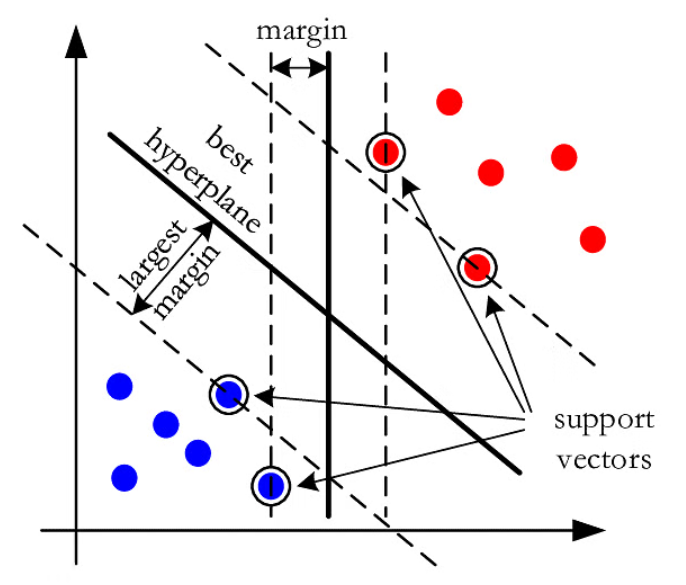
\includegraphics[width=0.55\linewidth]{SVM_Heart_Disease.png}
\end{figure}

\subsection{Depth-based Classifier}
Depth-based classifiers, such as decision trees and random forests, are powerful machine learning algorithms commonly used for both classification and regression tasks. Decision trees recursively partition the feature space based on individual feature values, providing an interpretable sequence of if-else conditions. However, they can over-fit when the tree grows too deep. In contrast, random forests are ensembles of decision trees trained on random subsets of the data and features, mitigating overfitting by aggregating predictions. Both algorithms find applications in classification and regression tasks, with decision trees being interpretable and random forests offering enhanced generalization capabilities.

\subsection{Kernel Density Function-based Classifier}
Kernel density-based classifiers are non-parametric techniques used for density estimation and classification tasks. In classification, kernel density estimation is used to model the conditional probability distributions of different classes, and the class of a new data point is determined based on which class has the highest density at that point. Kernel density-based classifiers are particularly useful when dealing with data distributions that are not easily modeled by parametric methods and can handle complex, multi-modal data distributions.


\subsection{KNN-based Classifier}
The k-Nearest Neighbors (k-NN) algorithm is a versatile machine learning technique used for classification and regression tasks. It determines the class or predicts the value of a new data point by examining the labels or values of its k nearest neighbors in the feature space, based on a distance metric such as Euclidean distance. While simple to implement and understand, k-NN's computational cost can be high for large datasets, and the choice of the parameter k is crucial for its performance.

\section{Comparing Different Machine Learning Models}
Comparing different machine learning models involves evaluating their performance using various metrics and then selecting the model that performs the best according to your criteria. We'll be making confusion matrix for all the models and calculate it's accuracy, precision, recall and F1 score.

\begin{itemize}
    \item \textbf{Accuracy}: Accuracy measures the proportion of correct predictions among the total number of predictions. It gives an overall measure of correctness but may not be suitable for imbalanced datasets. It's calculated as: 
$$Accuracy = \frac{True\ Positives + True\ Negatives}{True\ Positives + True\ Negatives + False\ Positives + False\ Negatives}$$
\item \textbf{Precision}: Precision measures the proportion of true positive predictions among the total number of positive predictions. It provide insights into how well the model identifies positive instances and avoids false positives. It's calculated as: 
$$Precision = \frac{True\ Positives}{True\ Positives + False\ Positives}$$
\item \textbf{Recall(Sensitivity)} Recall measures the proportion of true positive predictions among the total number of actual positive instances. It provide insights into how well the model identifies positive instances and avoids false negatives. It's calculated as:
$$Recall = \frac{True\ Positives}{True\ Positives + False\ Negatives}$$
\item \textbf{F1 Score}: The F1 score is the harmonic mean of precision and recall. It provides a single score that balances both precision and recall. It balances precision and recall and can be useful when you want to consider both false positives and false negatives. 
It's calculated as:
$$F1 \ Score = 2 \times \frac{Precision \times Recall}{Precision + Recall}$$
\end{itemize}
\noindent As in our case we want to minimize chances of a false positives as they can lead to unnecessary anxiety, additional medical tests, treatments, and healthcare costs for patients who do not have the disease. So we are gonna prioritize on increasing precision along with accuracy.

\section{Different Machine Learning Approaches on Heart Disease Dataset}
To test out the how different models perform on this task, we will be using the \textbf{UCI Heart Disease} having 14 features and 303 samples.

We load our dataset and first of all we check for any missing values, as there are missing values present in this dataset we'll replace all the missing values of both features(having missing values) by their respective mode values.

\noindent The first few samples of dataset are as follows:
\begin{figure}[h]
    \centering
    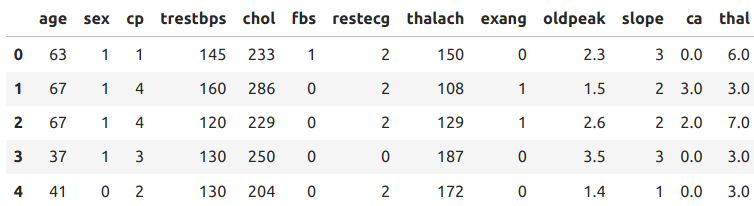
\includegraphics[width=0.75\linewidth]{before.png}
\end{figure}

\noindent We see that some of them are categorical variables. The basics of feature engineering and data science tell us that such columns need to be encoded to avoid unintentional bias. For example, as shown below, columns like chest pain (cp), restecg, slope, ca and thal need to be one-hot encoded in addition to others. Moreover, the columns of age, cholesterol (chol), Rest BP (trestbps), thalach, and oldpeak need to be normalized.

After applying one hot-encoding and normalization the dataset looks like the below:
\begin{figure}[h]
\centering
    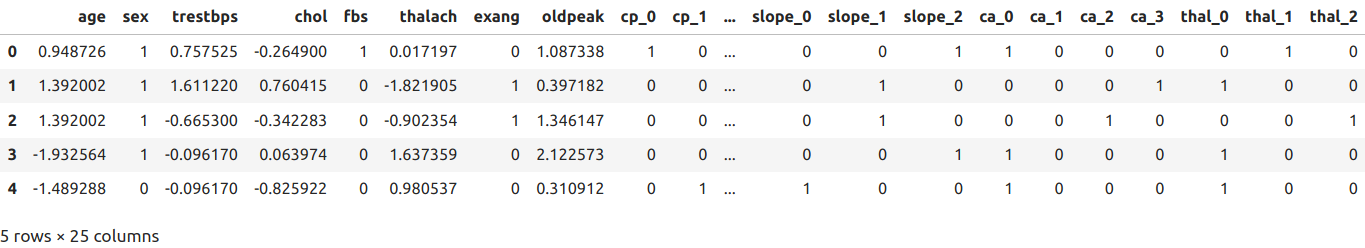
\includegraphics[width=\linewidth]{after.png}
\end{figure}

\noindent Then we trained our various machine learning models on this normalized dataset with a train-test split of 80\% to 20\% of original samples respectively.

\subsection{SVM-based Classifier}
The svm.SVC function in sklearn has several hyperparameters. We explored the primary ones i.e. choice of kernel(linear, poly, rbf and sigmoid), regularization parameter, and degree of the polynomial kernel and we found that the best kernel choice is 'RBF', with regularization parameter being 2.0.
This choice of hyperparameters gives 88.5\% accuracy and 90.3\% precision on the test set.
\begin{figure}[h]
\centering
    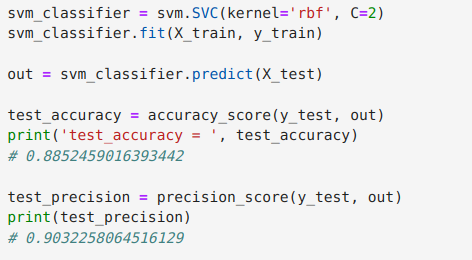
\includegraphics[width=0.55\linewidth]{svm.png}
\end{figure}

\subsection{Depth-based Classifier}
For Depth based classifer we used Random Forest Classifier, and calculated the accuracy on test set for various values of the n estimators parameter on tree level.

\begin{figure}[h]
\centering
    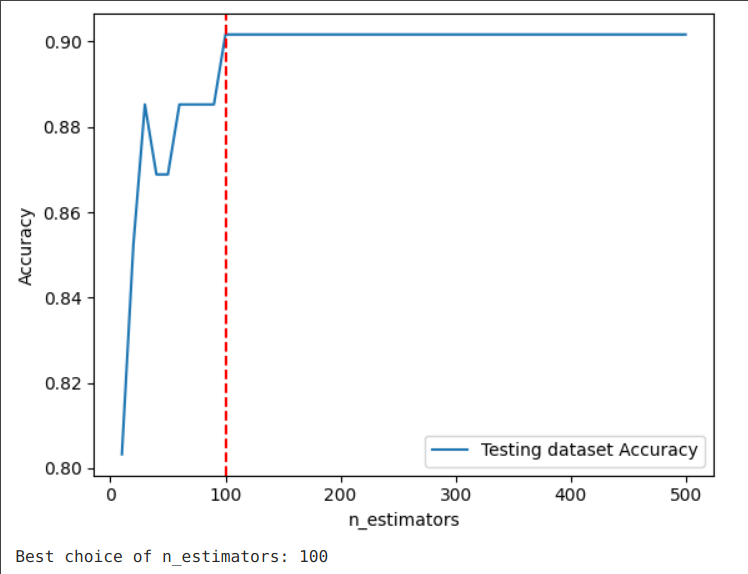
\includegraphics[width=0.75\linewidth]{randomforest.png}
\end{figure}

\noindent With the choice of 100 estimators, our random forest classifier gives around 90.1\% accuracy  and 93.3\% precision on the test set.
\begin{figure}[h]
\centering
    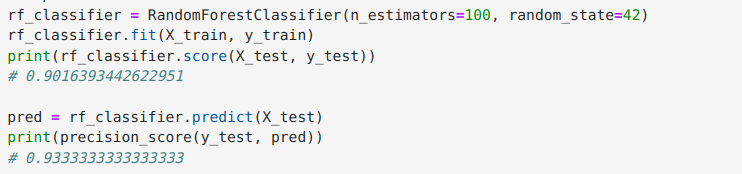
\includegraphics[width=0.75\linewidth]{rf.png}
\end{figure}

\subsection{Kernel Density based Classifier}
We first seperated our training dataset on the bases of target class and applied Kernel density model on it. When a new data point comes it is assigned the class on the basis of the density of that point in both of the classes.

\begin{figure}[h]
\centering
    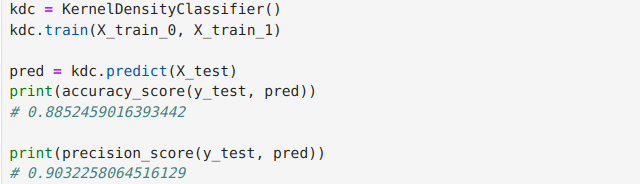
\includegraphics[width=0.75\linewidth]{kdc.png}
\end{figure}
\noindent Kernel Density Classifier gives us around 88.5\% accuracy 
 and 90.3\% precision on test set.

\subsection{KNN based Classifier}
Using the KNeighborsClassifier module from sklearn, we build a KNN model and iteratively tune the hyperparameter n-neighbors (number of neighbours to be checked for every data point).

\begin{figure}[h]
\centering
    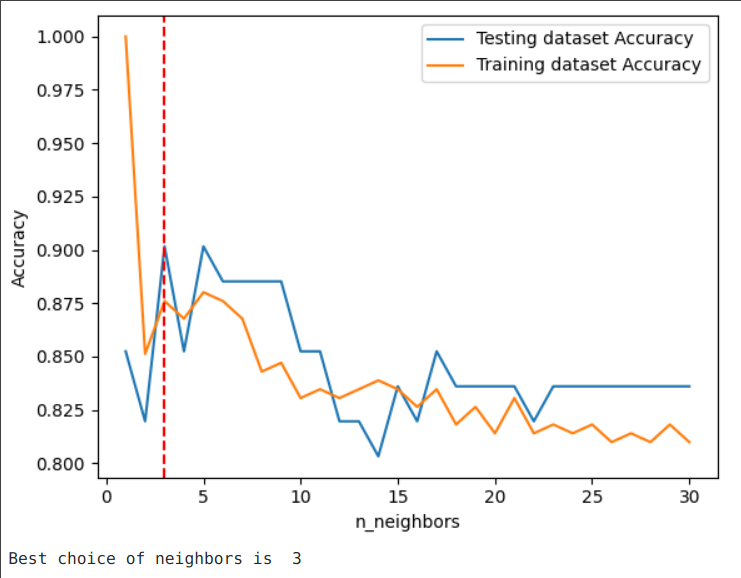
\includegraphics[width=0.75\linewidth]{knngraph.png}
\end{figure}
\noindent We see that the best choice of K is 3, and the accuracy and precision of this model is around 90.2\% and 93.3\% respectively.
\begin{figure}[h]
\centering
    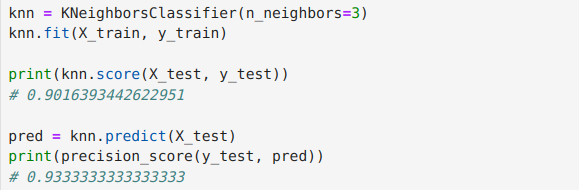
\includegraphics[width=0.75\linewidth]{knn.png}
\end{figure}
\newpage
\subsection{Box plots on Precision of various model}
Now we check the Precision of our final models at different splits of our dataset like 90/10, 80/20, 70/30, 60/40 and 50/50.
The we make a box plot out of them.
\begin{figure}[h]
\centering
    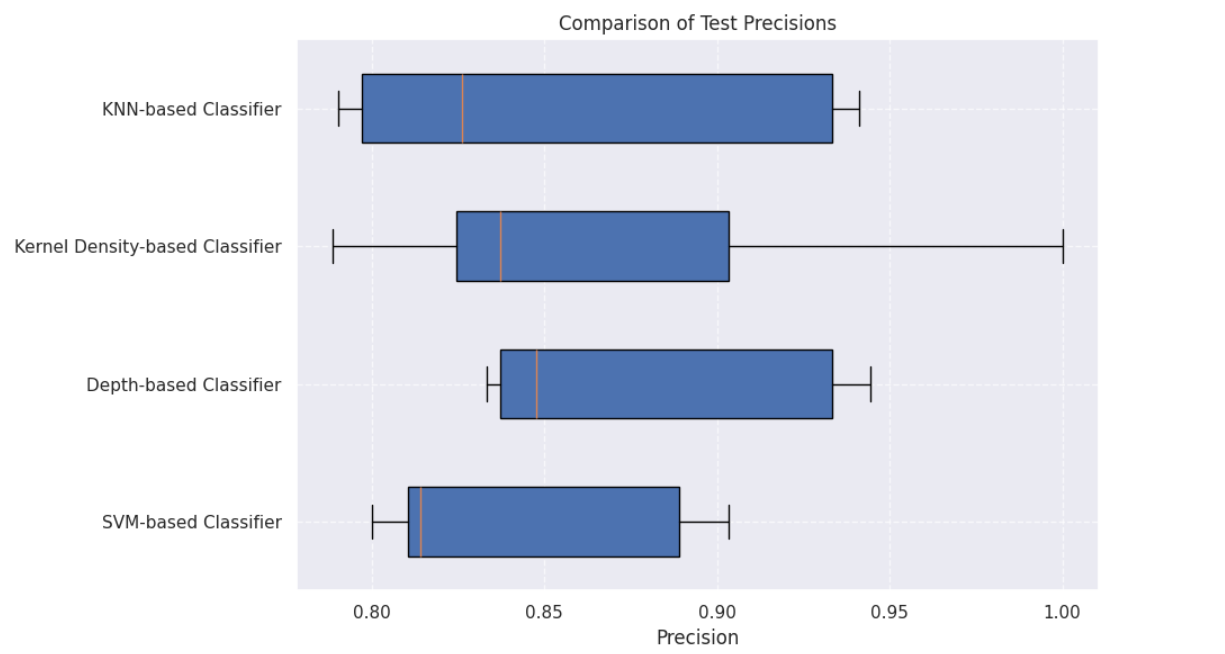
\includegraphics[width=0.9\linewidth]{PrecisionBox.png}
\end{figure}


\subsection{Box plots on Accuracy of various model}
Now we check the accuracy of our final models at different splits of our dataset like 90/10, 80/20, 70/30, 60/40 and 50/50.
The we make a box plot out of them.
\begin{figure}[h]
\centering
    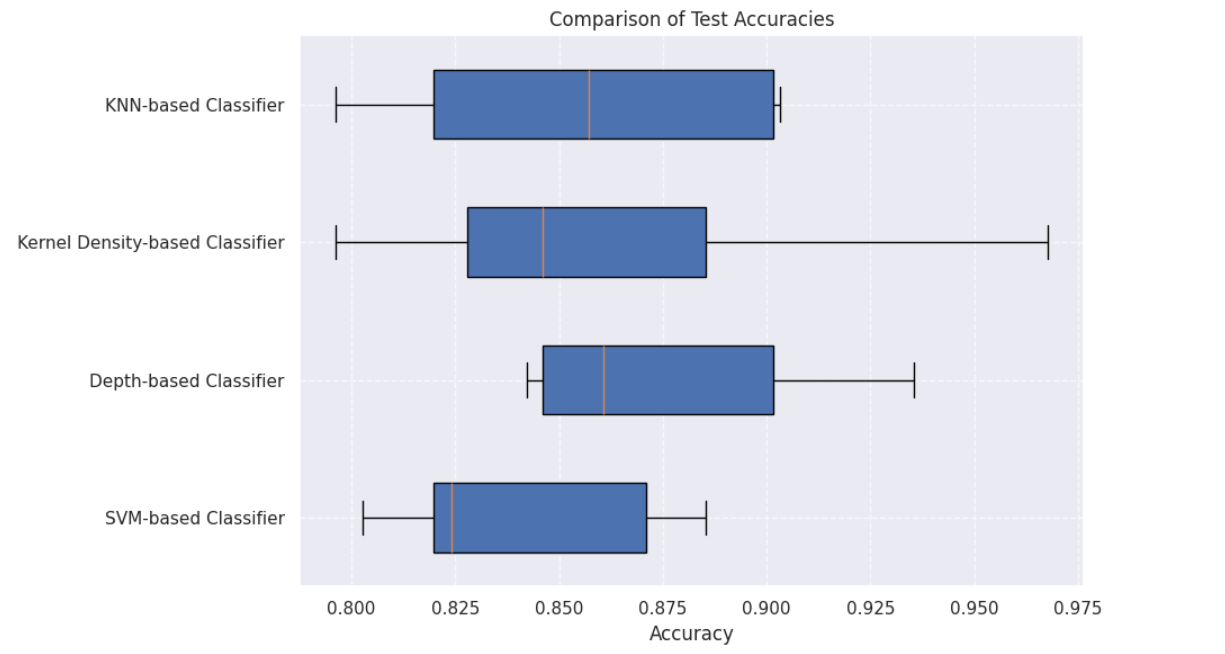
\includegraphics[width=0.9\linewidth]{AccuracyBox.png}
\end{figure}

\noindent After trying four different machine learning techniques to predict heart disease, it is clear that \textbf{Depth Based(Random Forest) Classifier} perform the best on average on our UCI dataset. However, feature engineering and hyperparameter tuning in other models can also yield comparable results.

\end{document}
